\documentclass{article}

\usepackage{fancyhdr}
\usepackage{extramarks}
\usepackage{amsmath}
\usepackage{amsthm}
\usepackage{amsfonts}
\usepackage{tikz}
\usepackage[plain]{algorithm}
\usepackage{algpseudocode}
\usepackage{tikz,pgfplots,multicol}
\usepackage[font=small,labelformat=empty]{caption}
\usetikzlibrary{automata,positioning}

%
% Basic Document Settings
%

\topmargin=-0.45in
\evensidemargin=0in
\oddsidemargin=0in
\textwidth=6.5in
\textheight=9.0in
\headsep=0.25in

\linespread{1.1}

\pagestyle{fancy}
\lhead{\hmwkAuthorName}
\chead{\hmwkClass\ (\hmwkClassInstructor\ \hmwkClassTime)}
\rhead{\hmwkTitle}
\lfoot{\lastxmark}
\cfoot{\thepage}

\renewcommand\headrulewidth{0.4pt}
\renewcommand\footrulewidth{0.4pt}

\setlength\parindent{0pt}

\setcounter{secnumdepth}{0}
\newcounter{partCounter}
\newcounter{homeworkProblemCounter}
\setcounter{homeworkProblemCounter}{1}
\nobreak\extramarks{Problem \arabic{homeworkProblemCounter}}{}\nobreak{}

%
% Homework Problem Environment
%
% This environment takes an optional argument. When given, it will adjust the
% problem counter. This is useful for when the problems given for your
% assignment aren't sequential. See the last 3 problems of this template for an
% example.
%
\newenvironment{homeworkProblem}[1][-1]{
    \ifnum#1>0
        \setcounter{homeworkProblemCounter}{#1}
    \fi
    \section{Problem \arabic{homeworkProblemCounter}}
    \setcounter{partCounter}{1}
    \enterProblemHeader{homeworkProblemCounter}
}{
    \exitProblemHeader{homeworkProblemCounter}
}

%
% Homework Details
%   - Title
%   - Due date
%   - Class
%   - Section/Time
%   - Instructor
%   - Author
%

\newcommand{\hmwkTitle}{HW \#4}
\newcommand{\hmwkDueDate}{February 9, 2017}
\newcommand{\hmwkClass}{MATH 1300}
\newcommand{\hmwkClassTime}{Section 005}
\newcommand{\hmwkClassInstructor}{Professor Braden Balentine}
\newcommand{\hmwkAuthorName}{\textbf{John Keller}}

%
% Title Page
%

\title{
    \vspace{2in}
    \textmd{\textbf{\hmwkClass:\ \hmwkTitle}}\\
    \normalsize\vspace{0.1in}\small{Due\ on\ \hmwkDueDate\ at 10:00am}\\
    \vspace{0.1in}\large{\textit{\hmwkClassInstructor\ \hmwkClassTime}}
    \vspace{3in}
}

\author{\hmwkAuthorName}
\date{}

\renewcommand{\part}[1]{\textbf{\large Part \Alph{partCounter}}\stepcounter{partCounter}\\}

%
% Various Helper Commands
%

% Useful for algorithms
\newcommand{\alg}[1]{\textsc{\bfseries \footnotesize #1}}

% For derivatives
\newcommand{\deriv}[1]{\frac{\mathrm{d}}{\mathrm{d}x} (#1)}

% For partial derivatives
\newcommand{\pderiv}[2]{\frac{\partial}{\partial #1} (#2)}

% Integral dx
\newcommand{\dx}{\mathrm{d}x}

% Alias for the Solution section header
\newcommand{\solution}{\textbf{\large Solution}}

% Probability commands: Expectation, Variance, Covariance, Bias
\newcommand{\E}{\mathrm{E}}
\newcommand{\Var}{\mathrm{Var}}
\newcommand{\Cov}{\mathrm{Cov}}
\newcommand{\Bias}{\mathrm{Bias}}

\begin{document}

\maketitle

\pagebreak

\section{Interpretation of Derivatives}

\begin{enumerate}
\setcounter{enumi}{0}
	\item Let $V(t)$ be the volume of water in a tank (in liters), at time $t$ (in seconds).
	\begin{enumerate}
		\item What are the meaning and units of $\frac{dV}{dt}$?\newline
			This means the derivative on the curve of liters vs. seconds of water in the tank. The units are liters per second.
		\item The tank is full at time $t_0$, so that $V(t_0)>0$. At some later time $t_1$ a drain is opened 20 cm above the bottom of the tank (which is taller than 20 cm), emptying water from side of the tank. Is $\frac{dV}{dt}$ positive, negative, or zero
			\begin{enumerate}
				\item at times $t$ with $t_0 < t < t_1$?\newline
					Negative.
				\item after the drain has been opened at $t_1$, but before the water has dropped to 20 cm above the bottom of the tank?\newline
					Negative.
				\item after the water drops to the drain hole 20 cm above the bottom of the tank?\newline
					Zero.
			\end{enumerate}
	\end{enumerate}
	\item Let $f(t)$ be the amount of rain in cm, that has fallen since midnight, with $t$ measured in hours. Interpret the following in practical terms, giving units:
	\begin{enumerate}
		\item $f(7)=2.4$\newline
			At 7 hours past midnight, there has been 2.4 cm total of rain that has fallen.
		\item $f'(7)=0.21$\newline
			At exactly 7 hours past midnight, the rain is falling at approximately 0.21 cm per hour.
		\item $f^{-1}(3)=12.3$\newline
			At $\frac{1}{3}$ hour past midnight, 12.3 cm of total rain has fallen.
		\item $(f^{-1})'(3)=86$\newline
			At exactly $\frac{1}{3}$ hour past midnight, the rain is falling at approximately 86 cm per hour.
	\end{enumerate}
\end{enumerate}

\section{Section 2.5}
\begin{enumerate}
\setcounter{enumi}{5}
	\item Sketch a graph of an example of a function $f$ that satisfies all of the given conditions $$\underset{x \rightarrow 2}{\text{lim}}f(x)=\infty, \quad \underset{x \rightarrow -2^+}{\text{lim}}f(x)=\infty, \quad \underset{x \rightarrow -2^-}{\text{lim}}f(x)=-\infty,\quad \newline
		\underset{x \rightarrow -\infty}{\text{lim}}f(x)=0, \quad \underset{x \rightarrow \infty}{\text{lim}}f(x)=0, \quad f(0)=0$$
	
	\begin{center}
		\pgfplotsset{width=0.9\linewidth,height=8cm}
%		\pgfplotsset{xmin=-10,xmax=10,ymin=-4,ymax=6,soldot/.style={color=blue,only marks,mark=*}
			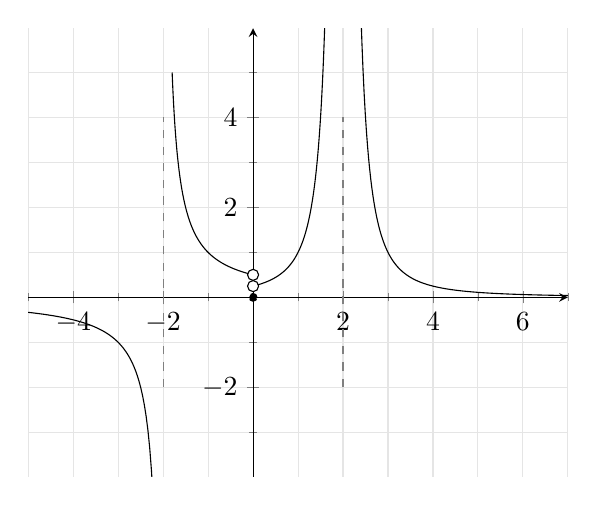
\begin{tikzpicture}
			\begin{axis}[ymin=-2,ymax=4,xmin=-5,xmax=7,axis lines=middle,axis equal,grid=both,minor tick num=1,grid style={solid, gray!20}]
				\addplot[samples=200,domain=-10:-2.1] {(1)/(x+2)};
				\addplot[samples=200,domain=-1.8:0] {(1)/(x+2)};
				\addplot[samples=200,domain=0:1.9] {(1)/((x-2)^2)};
				\addplot[samples=200,domain=2.1:7] {(1)/((x-2)^2)};
				\addplot+[only marks,mark=*,mark options={fill=white},text mark as node=false,black] coordinates {(0,0.5)(0,0.25)};
				\addplot+[only marks,mark=*,mark options={fill=black,scale=0.7},text mark as node=false,black] coordinates {(0,0)};
				\addplot[domain=0:6,gray,dashed] coordinates {(2,-2)(2,4)};
				\addplot[domain=-5:6,gray,dashed] coordinates {(-2,-2)(-2,4)};
			\end{axis}
		\end{tikzpicture}
		\end{center}
	
\setcounter{enumi}{25}
	\item Find the limit: 
	$$\begin{aligned}
		&\underset{x \rightarrow \infty}{\text{lim}}\frac{x+2}{\sqrt{9x^2+1}}\\
		&\underset{x \rightarrow \infty}{\text{lim}}\frac{1+\frac{2}{x}}{\sqrt{\frac{1}{x^2}+9}}\\
		&\frac{\underset{x \rightarrow \infty}{\text{lim}}(1+\frac{2}{x})}{\underset{x \rightarrow \infty}{\text{lim}}(\sqrt{\frac{1}{x^2}+9})} = \frac{\underset{x \rightarrow \infty}{\text{lim}}(1)+\underset{x \rightarrow \infty}{\text{lim}}(\frac{2}{x})}{\sqrt{\underset{x \rightarrow \infty}{\text{lim}}(\frac{1}{x^2})+\underset{x \rightarrow \infty}{\text{lim}}(9)}}= \frac{1}{\sqrt{9}}=\frac{1}{3}\\
	\end{aligned}$$
\setcounter{enumi}{31}
	\item Find the limit: 
	$$\begin{aligned}	
		&\underset{x \rightarrow \infty}{\text{lim}}\frac{\sin^2x}{x^2}\\
		-1 \leq &\sin(x) \leq 1\\
		\underset{x \rightarrow \infty}{\text{lim}}\Big(\frac{0}{x^2}\Big) \leq &\underset{x \rightarrow \infty}{\text{lim}} \Big(\frac{\sin^2 x}{x^2}\Big)\leq \underset{x \rightarrow \infty}{\text{lim}} \Big(\frac{1}{x^2}\Big)\\
		0 \leq &\underset{x \rightarrow \infty}{\text{lim}} \Big(\frac{\sin^2 x}{x^2}\Big)\leq 0
	\end{aligned}$$
	Therefore, by the \textbf{squeeze theorem}, because $\underset{x \rightarrow \infty}{\text{lim}}\Big(\frac{0}{x^2}\Big)=0$, then $\underset{x \rightarrow \infty}{\text{lim}}\frac{\sin^2x}{x^2}$ must be $0$.
\setcounter{enumi}{47}
	\item Find a formula for a function that has vertical asymptotes $x=1$ and $x=3$ and a horizontal asymptote at $y=1$.
		\begin{center}
		\begin{minipage}{.3\textwidth}
		\begin{center}
			$$f(x)=\frac{x-2}{(x-2)^2-1}+1$$
		\end{center}
		\end{minipage}% <---------------- Note the use of "%"
		\begin{minipage}{.7\textwidth}
		
		\begin{center}
		\pgfplotsset{width=0.9\linewidth,height=5cm}
%		\pgfplotsset{xmin=-10,xmax=10,ymin=-4,ymax=6,soldot/.style={color=blue,only marks,mark=*}
			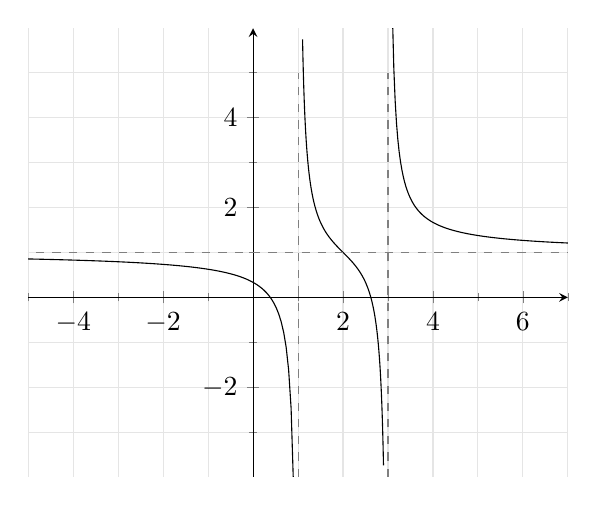
\begin{tikzpicture}
			\begin{axis}[ymin=-2,ymax=4,xmin=-5,xmax=7,axis lines=middle,axis equal,grid=both,minor tick num=1,grid style={solid, gray!20}]
				\addplot[samples=200,domain=-10:0.9] {(x-2)/((x-2)^2-1)+1};
				\addplot[samples=200,domain=1.1:2.9] {(x-2)/((x-2)^2-1)+1};
				\addplot[samples=200,domain=3.1:9] {(x-2)/((x-2)^2-1)+1};
				\addplot[domain=-10:10,gray,dashed] {1};
				\addplot[domain=0:6,gray,dashed] coordinates {(1,-4)(1,5)};
				\addplot[domain=0:6,gray,dashed] coordinates {(3,-4)(3,5)};
			\end{axis}
		\end{tikzpicture}
		\end{center}
		\end{minipage}
		\end{center}
		
		
\setcounter{enumi}{54}
	\item \begin{enumerate}
		\item A tank contains 5000 L of pure water brine that contains 30 g of salt per liter of water is pumped into the tank at a rate of 25 L/min. Show that concentration of salt after $t$ minutes (in grams per liter) is $$C(t)=\frac{30t}{200+t}$$
		$$\begin{align}
			C(t)&= 5000 \cdot \Big(\frac{30\text{ g of salt}}{1\text{ L of water}}\Big) \cdot \Big(\frac{25\text{ L of water}}{1\text{ minute}}\Big)\\
		\end{align}$$
		\item What happens to the concentration as $t\rightarrow \infty$?\newline
			The concentration approaches 30 grams per liter.
	\end{enumerate}
\end{enumerate}
	
\section{Section 2.6}
\begin{enumerate}
\setcounter{enumi}{11}
	\item Shown are graphs of the position of functions of two runners, A and B, who run a 100-m race and finish in a tie. \begin{center}\includegraphics[width=6cm]{images/26pr12}\end{center}
	\begin{enumerate}
		\item Describe and compare how the runners run the race. \newline
			Both runners had different strategies, but got to the 100-m finish at the same time. Runner A decided to keep the exact same speed throughout the entire race, which is pretty unbelievable. Runner B was much more realistic, and started at a slower speed, steadily increasing it throughout. It is likely that Runner A began before the start line, as it is impossible to go from 0 to full speed instantaneously.
		\item At what time is the distance between the runners the greatest?\newline
			The time at which the distance between the runners is greatest is at approximately 9 seconds, when the runners are about 40-m apart.
		\item At what time do they have the same velocity?\newline
			The runners have the same velocity the second they cross the finish line, at 14 seconds into the race.
	\end{enumerate}
\setcounter{enumi}{16}
	\item For the function $g$ whose graph is given, arrange the following numbers in increasing order and explain your reasoning: $$0 \qquad g'(-2) \qquad g'(0) \qquad g'(2) \qquad g'(4)$$
	\begin{center}\includegraphics[width=6cm]{images/26pr17}\end{center}
	$$g'(0)<0<g'(4)<g'(2)<g'(-2)$$
	To arrange the above values by order, I first determined which prime values were less than 0, and it turned out only $g'(0)$ is negative. Then I determined which lines have a greater tangent slope by visualizing a tangent line at each of the points listed.
\pagebreak
\setcounter{enumi}{20}
	\item Sketch the graph of a function $f$ for which $f(0)=0, f'(0)=3, f'(1)=0, \text{ and } f'(2)=-1$
	\begin{center}
		\pgfplotsset{width=0.8\linewidth,height=7cm}
%		\pgfplotsset{xmin=-10,xmax=10,ymin=-4,ymax=6,soldot/.style={color=blue,only marks,mark=*}
			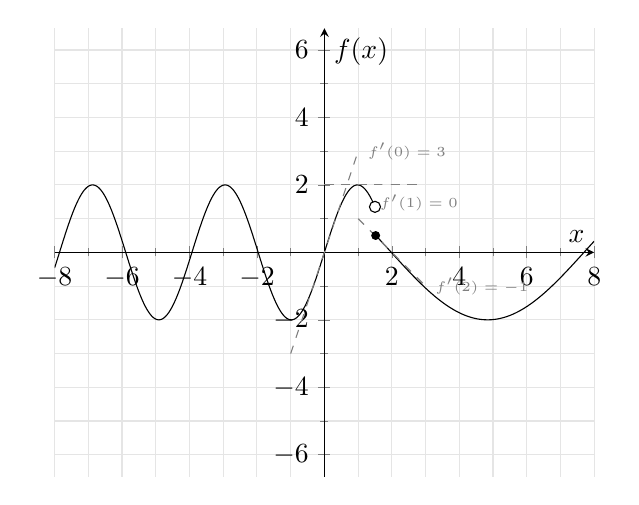
\begin{tikzpicture}
			\begin{axis}[axis lines=middle,xlabel=$x$,ylabel=$f(x)$,axis equal,grid=both,minor tick num=1,grid style={solid, gray!20}]
				\addplot[samples=500,domain=-8:1.5] {2*sin(deg(1.6*x))};
				\addplot[samples=500,domain=1.5:8] {2*sin(deg(0.55*x+2.05))};
				\addplot+[only marks,mark=*,mark options={fill=white},text mark as node=false,black] coordinates {(1.5,1.35)};
				\addplot+[only marks,mark=*,mark options={fill=black,scale=0.7},text mark as node=false,black] coordinates {(1.52,0.5)};
				\addplot[domain=-1:1,gray,dashed] {3*x+0} node[right,pos=1] {\tiny{${f'(0)=3}$}};
				\addplot[samples=500,domain=0:2.8,gray,dashed] {2} node[below,pos=1] {\tiny{$f'(1)=0$}};
				\addplot[domain=1:3,gray,dashed] {-1*x+2} node[right,pos=1] {\tiny{$f'(2)=-1$}};
			\end{axis}
		\end{tikzpicture}
	\end{center}
\setcounter{enumi}{29}
	\item Find $f'(a)$ using the limit definition of derivative: $$f(x)=x^{-2}$$\newline
		$$\begin{align}
			f'(a)&=\underset{h\rightarrow 0}{\text{lim}}\frac{(x+h)^{-2}-(x^{-2})}{h}\\
			&=\underset{h\rightarrow 0}{\text{lim}}\ \frac{\frac{2}{x+h}-\frac{2}{x}}{h}\\
			&=\underset{h\rightarrow 0}{\text{lim}}\ \frac{\frac{2}{x+h}-\frac{2+h}{x+h}}{h}\\
			&=\underset{h\rightarrow 0}{\text{lim}}\ \frac{\frac{-h}{x+h}}{h}\\
			&=\underset{h\rightarrow 0}{\text{lim}}\ \frac{2h}{xh(x+h)}\\
			&=\underset{h\rightarrow 0}{\text{lim}}\ \frac{2}{x(x+h)}\\
			&=\frac{2}{x(x+0)}\\
			&=\boxed{\frac{2}{x^2}}
		\end{align}$$
\end{enumerate}
\pagebreak
\section{Section 2.7}
\begin{enumerate}
\setcounter{enumi}{9}
	\item Trace or copy the graph of the given function $f$. (Assume that the axes have equal scales.) Then use the method of Example 1 to sketch the graph $f'$ below it.
	\begin{center}
	\begin{minipage}[t]{.5\textwidth}
	\begin{center}\includegraphics[width=3.4cm]{images/27pr10}\end{center}
	\captionof{figure}{$f(x)$}
	\end{minipage}% <---------------- Note the use of "%"
	\begin{minipage}[t]{.5\textwidth}
	\begin{center}\includegraphics[width=3.4cm]{images/27pr10a}\end{center}
	\captionof{figure}{$f'(x)$}
	\end{minipage}
	\end{center}
\setcounter{enumi}{33}
	\item Let $P(t)$ be the percentage of Americans under the age of 18 at time $t$. The table gives values of this function in census years from 1950 to 2000.
	\begin{center}
		\begin{tabular}{c|c}
		$t$    & $P(t)$ \\\hline
		1950 & 31.1 \\
		1960 & 35.7 \\
		1970 & 34.0 \\
		1980 & 28.0 \\
		1990 & 25.7 \\
		2000 & 25.7
		\end{tabular}
	\end{center}
	\begin{enumerate}
		\item What is the meaning of $P'(t)$? What are its units? \newline
			The meaning of $P'(t)$ is simply the rate at which the number of people under 18 is decreasing or increasing every year. The units would likely be $t$ in years (considering the census is done annually), and $P(t)$ in millions of kids.
		\item Construct a table of estimated values for $P'(t)$.
			\begin{center}
				\begin{tabular}{c|c}
				$t$    & $P(t)$  \\\hline
				1955 & 32 \\
				1965 & 34.5 \\
				1975 & 30 \\
				1985 & 21 \\
				1995 & 35 \\
				2005 & 26
				\end{tabular}
			\end{center}
		\pagebreak
		\item Graph $P$ and $P'$.
			\begin{center}
			\pgfplotsset{compat=1.8,width=0.6\linewidth,height=7cm}
			
 			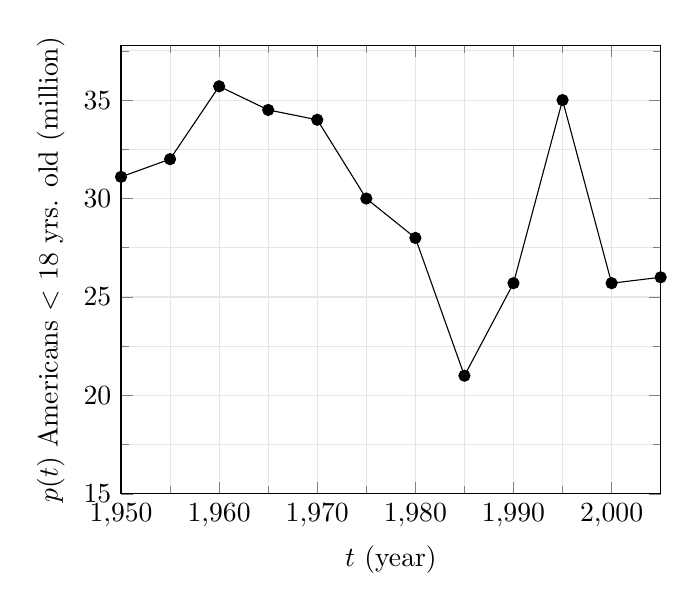
\begin{tikzpicture}
				\begin{axis}[xmin=1950,xmax=2005,ymin=15,xlabel=$t$ (year),ylabel=$p(t)$ Americans $<$ 18 yrs. old (million),grid=both,minor tick num=1,grid style={solid, gray!20}]
					\addplot+[mark=*,scale=0.5,mark options={fill=black},text mark as node=true,black] coordinates {
					    (1950,31.1)
					    (1955,32)
					    (1960,35.7)
					    (1965,34.5)
					    (1970,34)
					    (1975,30)
					    (1980,28)
					    (1985,21)
					    (1990,25.7)
					    (1995,35)
					    (2000,25.7)
					    (2005,26)};
				\end{axis}
			\end{tikzpicture}
			\end{center}
		\item How would it be possible to get more accurate values for $P'(t)$?\newline
			The obvious method would be to look up the data on the census website, but practically speaking the best way to get more accurate data would be to increase the frequency for which the data is recorded (for example every year instead of every 5).
	\end{enumerate}
\end{enumerate}

\end{document}